\documentclass[../../main.tex]{subfiles}

\graphicspath{{../../image/}{../../figure/}}

\begin{document}

\section{一个教学示例}\label{section:ch01-一个教学示例}

对机器学习领域的新人来说，许多基本概念和术语可以通过一个简单的例子来引入——用多项式拟合一个小型合成数据集（Bishop, 2006）。这是一个监督学习问题，在这个问题中，我们希望根据输入的变量值，对目标变量进行预测。

\subsection{合成数据}\label{subsection:ch01-合成数据}

我们用 $x$ 表示输入变量，用 $t$ 表示目标变量，并假设这两个变量在实数轴上取值连续。给定一个训练集，其中包含 $N$ 个 $x$ 的观测值，记作 $x_1,\cdots,x_N$，还包含相应 $t$ 的观测值，记作 $t_1,\cdots,t_N$。我们的目标是根据 $x$ 的某个新值来预测相应的 $t$ 的值。机器学习的一个关键目标是对以前未见过的输入进行准确预测，这种能力称为泛化能力（generalization）。

\begin{definition}[泛化能力]\label{definition:ch01-泛化能力}
设输入空间 $\mathcal{X}\subseteq\mathbb{R}^{D}$（$D\in\mathbb{N}$），目标空间 $\mathcal{Y}\subseteq\mathbb{R}$，训练集 $\mathcal{D}=\{(x_n,t_n)\}_{n=1}^{N}$（$N\in\mathbb{N}$），模型 $y(\cdot;\mathbf{w}):\mathcal{X}\to\mathcal{Y}$ 的权重 $\mathbf{w}\in\mathcal{W}\subseteq\mathbb{R}^{P}$（$P\in\mathbb{N}$）由 $\mathcal{D}$ 确定；设损失函数 $\ell:\mathcal{Y}\times\mathcal{Y}\to[0,\infty)$，$(\Omega,\mathcal{F},\mathbb{P})$ 为概率空间，$(X,T):\Omega\to\mathcal{X}\times\mathcal{Y}$ 与 $\mathcal{D}$ 独立同分布，且 $\mathbb{E}\bigl[\ell(y(X;\mathbf{w}),T)\bigr]<\infty$。记
\begin{align*}
  \widehat{R}_{\mathcal{D}}(\mathbf{w})=\frac{1}{N}\sum_{n=1}^{N}\ell\bigl(y(x_n;\mathbf{w}),t_n\bigr),
  \qquad
  R(\mathbf{w})=\mathbb{E}\bigl[\ell\bigl(y(X;\mathbf{w}),T\bigr)\bigr],
\end{align*}
分别称为\textbf{训练误差}与\textbf{泛化误差}，并称 $R(\mathbf{w})-\widehat{R}_{\mathcal{D}}(\mathbf{w})$ 为\textbf{泛化间隙}（generalization gap）。设 $\varepsilon>0$。若
\begin{enumerate}
  \item $R(\mathbf{w})\leqslant\varepsilon$，即模型在未参与训练的样本上的期望损失不超过 $\varepsilon$；
  \item $R(\mathbf{w})-\widehat{R}_{\mathcal{D}}(\mathbf{w})\leqslant\varepsilon$，即泛化间隙不超过 $\varepsilon$，
\end{enumerate}
则称 $y(\cdot;\mathbf{w})$ 具有 $\varepsilon$-\textbf{泛化能力}（generalization）。
\end{definition}

% SUPPLEMENT: parent=definition:ch01-泛化能力; kind=motivation; location=紧随其后的 remark
\begin{remark}
这里的关键限定是“训练集以外”。若一个输入本来就在训练数据之中，模型对它给出正确回答只说明它记住了这个样本，并不构成泛化；因此本书后面的做法总是：预留一部分与训练集不相交的数据，只在这些数据上衡量预测是否准确。
还有一点需要澄清：泛化能力是相对于“数据由什么规律产生、模型见过多少数据”而言的性质，而不是模型单独具有的属性。同一个模型在小训练集上可能泛化很差，在更大的训练集上却泛化良好，这正是\cref{subsection:ch01-模型复杂度}中要定量考察的现象。
\end{remark}

我们可以通过从正弦函数采样生成的合成数据集来说明这一点。

\begin{example}[ 正弦合成数据集]\label{example:ch01-正弦合成数据集}
取 $N=10$。输入值 $x_n$（$n=1,\cdots,N$）通过在区间 $[0,1]$ 上均匀采样生成；对应的目标值 $t_n$ 则是先计算每个 $x$ 所对应的函数 $\sin(2\pi x)$ 的值，然后向每个数据点添加少量随机噪声（由 Gauss 分布控制，参见\cref{section:ch02-Gauss分布}）得到的。
\end{example}

通过这种方式生成数据，我们可以捕获许多现实世界数据集的一个重要特性——它们具有我们希望了解的潜在规律，但个别观测值会被随机噪声干扰。这种噪声可能源于它们固有的随机过程（例如放射性衰变），但更常见的原因是存在未被观测到的变异源。

\begin{remark}
\cref{example:ch01-正弦合成数据集}把“噪声”这一步写得更具体些：若记 $t_n=\sin(2\pi x_n)+\varepsilon_n$，其中 $\varepsilon_n$ 是相互独立的随机变量，则 $\sin(2\pi x_n)$ 是决定观测的\textbf{系统性成分}，而 $\varepsilon_n$ 是\textbf{随机性成分}。本例中后者取为均值为 $0$ 的 Gauss 噪声，其标准差控制了圆点在曲线附近的散布程度。
这一分解的作用在于：它说明“从数据中学习”不是去解释每一个观测点，而是去估计那个系统性成分。若没有噪声，则在次数不超过 $N-1$ 的多项式中，通过这 $N$ 个点的那条曲线是唯一的；正因为有噪声，任何只依据有限样本的估计都会带有不确定性，这也是后文要用概率论（参见\cref{section:ch02-概率法则}）来刻画预测的原因。
\end{remark}

\begin{figure}[htbp]
  \centering
  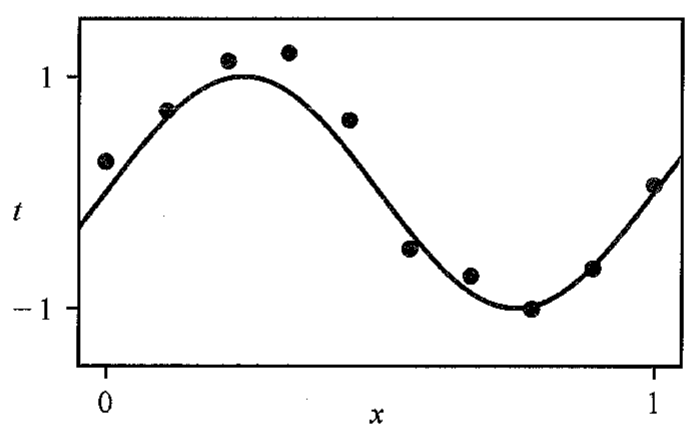
\includegraphics[width=0.62\textwidth]{ch01-fig1-5-sin-training.png}
  \caption{一个由 $N=10$ 个数据点组成的训练集，以蓝色圆点显示，其中每个数据点包含了输入变量 $x$ 及其对应的目标变量 $t$ 的观测值。绿色曲线显示了用来生成数据的函数 $\sin(2\pi x)$。我们的目标是在不知道绿色曲线的情况下，预测新的输入变量 $x$ 所对应的目标变量 $t$ 的值。}
  \label{figure:ch01-正弦拟合训练集}
\end{figure}

在这个示例中，我们事先知道真正生成数据是通过一个正弦函数。在机器学习的实际应用中，我们的目标是在有限的训练集中发现隐藏的规律。不过，了解数据的生成过程有助于我们阐明机器学习中的一些重要概念。

\subsection{线性模型}\label{subsection:ch01-线性模型}

现在让我们先从一种相对非正式的方式出发，考虑一种基于曲线拟合的简单方法。我们将使用多项式函数来拟合数据，其形式如下：

\begin{definition}[多项式模型]\label{definition:ch01-多项式模型}
设 $M\in\mathbb{N}$，$x\in\mathbb{R}$，$\mathbf{w}=(w_0,w_1,\cdots,w_M)\in\mathbb{R}^{M+1}$ 为实系数向量，其中 $w_j\in\mathbb{R}$ 为 $x^{j}$ 的系数（$j=0,1,\cdots,M$）。由
\begin{align}
  y(x,\mathbf{w}) = w_0 + w_1 x + w_2 x^2 + \cdots + w_M x^M = \sum_{j=0}^{M} w_j x^j
  \label{align:ch01-多项式模型}
\end{align}
给出的函数 $y(\cdot,\mathbf{w}):\mathbb{R}\to\mathbb{R}$ 称为\textbf{$M$ 阶多项式函数}，以它为预测函数、以 $\mathbb{R}^{M+1}$ 为参数空间的模型称为\textbf{多项式模型}（polynomial model）。其中 $M$ 称为多项式的\textbf{阶数}（order），$x^{j}$ 表示 $x$ 的 $j$ 次幂。若 $w_M\neq0$，则 $M$ 称为 $y(\cdot,\mathbf{w})$ 的\textbf{次数}（degree）；若 $w_M=0$，则 $y(\cdot,\mathbf{w})$ 等于某个阶数低于 $M$ 的多项式函数。
\end{definition}

% SUPPLEMENT: parent=definition:ch01-多项式模型; kind=motivation; location=紧随其后的 remark
\begin{remark}
引入多项式模型的动机是把“寻找一条曲线”换成“确定一个有限维向量”。未知函数有无穷多个自由度，而 $M$ 阶多项式只由 $M+1$ 个实数决定，于是“学习”就归结为从训练数据中把这 $M+1$ 个数定下来，这使问题可以用微积分与线性代数处理。
条件方面要注意两点。其一，$M$ 是模型的\textbf{结构参数}而不是待拟合的系数：给定 $M$，可选的函数族才被固定，因此 $M$ 不能靠最小化训练误差来选（见\cref{subsection:ch01-模型选择}）。其二，各阶函数族是\textbf{嵌套}的：$M$ 阶族包含全部低阶多项式（把高阶系数取 $0$ 即可），这一点在\cref{proposition:ch01-训练误差单调性}中会给出严格表述，它也是理解“$M=9$ 的训练误差不可能比 $M=3$ 差、测试误差却差得多”这一表面矛盾的出发点。
\end{remark}

注意，尽管多项式函数 $y(x,\mathbf{w})$ 是 $x$ 的非线性函数，但它也是系数 $\mathbf{w}$ 的线性函数。在式\eqref{align:ch01-多项式模型}中，像这个多项式一样，关于未知参数呈线性的函数具有重要的特性，同时也存在明显的局限性，它们被称为线性模型（linear model）。

\begin{definition}[线性模型]\label{definition:ch01-线性模型}
设输入空间 $\mathcal{X}\subseteq\mathbb{R}^{D}$（$D\in\mathbb{N}$），参数 $\mathbf{w}=(w_1,\cdots,w_{M})\in\mathbb{R}^{M}$（$M\in\mathbb{N}$），模型 $y(\cdot;\mathbf{w}):\mathcal{X}\to\mathbb{R}$。若存在与 $\mathbf{w}$ 无关的映射 $\phi_1,\cdots,\phi_{M}:\mathcal{X}\to\mathbb{R}$，使得对一切 $x\in\mathcal{X}$ 有
\begin{align*}
  y(x;\mathbf{w})=\sum_{j=1}^{M}w_j\,\phi_j(x),
\end{align*}
则 $y(\cdot;\mathbf{w})$ 称为关于参数 $\mathbf{w}$ 的\textbf{线性模型}（linear model），$\phi_j$ 称为\textbf{基函数}（basis function）。若存在与 $\mathbf{w}$ 无关的 $b:\mathcal{X}\to\mathbb{R}$ 使 $y(x;\mathbf{w})=b(x)+\sum_{j=1}^{M}w_j\phi_j(x)$，则 $y(x;\cdot)$ 关于 $\mathbf{w}$ 为仿射函数；此时把 $b$ 也作为待定参数、取 $\phi_0\equiv1$ 与 $w_0=b$，$y$ 即归入上述线性形式，故这种情形也称为线性模型。
\end{definition}

% SUPPLEMENT: parent=definition:ch01-线性模型; kind=motivation; location=紧随其后的 remark
\begin{remark}
“线性”修饰的是\textbf{对参数的依赖}，不是对输入 $x$ 的依赖：$x^M$、$\sin x$、$\log x$ 都可以作为输入特征进入线性模型，只要它们是已知的、不随 $\mathbf{w}$ 变化的函数。反过来，只要参数以乘积或复合的方式出现，就不再是线性模型。
这一区分的实际作用在于它决定了误差函数的面貌：若 $y$ 关于 $\mathbf{w}$ 是仿射的，则平方和误差是 $\mathbf{w}$ 的二次函数，其梯度是 $\mathbf{w}$ 的仿射函数，最小化问题有闭式解（\cref{proposition:ch01-最小二乘解}）；一旦失去对参数的线性，就只剩下迭代优化这一条路，这正是\cref{subsection:ch01-模型选择}末尾所说的现实困难，也是后续章节讨论梯度方法（参见\cref{section:ch07-梯度下降优化}）的原因。
\end{remark}

\subsection{误差函数}\label{subsection:ch01-误差函数}

多项式系数的值将通过拟合训练数据来确定，这可以通过最小化误差函数（error function）来实现，该误差函数度量了对于任意给定的 $\mathbf{w}$，函数 $y(x,\mathbf{w})$ 与训练集中数据点之间的拟合误差。

\begin{definition}[误差函数]\label{definition:ch01-误差函数}
设 $N\in\mathbb{N}$，训练集 $\mathcal{D}=\{(x_n,t_n)\}_{n=1}^{N}\subseteq\mathcal{X}\times\mathcal{Y}$，模型 $y(\cdot;\mathbf{w}):\mathcal{X}\to\mathcal{Y}$ 的参数 $\mathbf{w}\in\mathcal{W}\subseteq\mathbb{R}^{P}$（$P\in\mathbb{N}$），逐样本损失 $\ell:\mathcal{Y}\times\mathcal{Y}\to[0,\infty)$。若映射 $E:\mathcal{W}\to[0,\infty)$ 可写成
\begin{align*}
  E(\mathbf{w})=\sum_{n=1}^{N}\ell\bigl(y(x_n;\mathbf{w}),t_n\bigr),\qquad \mathbf{w}\in\mathcal{W},
\end{align*}
则 $E$ 称为训练集 $\mathcal{D}$ 上的\textbf{误差函数}（error function），$\ell$ 称为它的\textbf{逐样本损失}（pointwise loss）。$E$ 的取值只由训练集与模型决定，与检验数据无关。
\end{definition}

% SUPPLEMENT: parent=definition:ch01-误差函数; kind=motivation; location=紧随其后的 remark
\begin{remark}
误差函数的作用是把“拟合得好不好”这一模糊说法压缩成一个可以比较大小的实数，从而把学习问题转化为一个优化问题：在所有候选参数中取使 $E(\mathbf{w})$ 最小者。没有这一步，就无法谈论“最优”模型。
条件上，误差函数必须\textbf{只由训练集和模型决定}，不能依赖测试数据或任何未知量；同时，为了能用基于梯度的算法（\cref{section:ch07-梯度下降优化}）求解，通常还要求它对 $\mathbf{w}$ 可微。不同的误差函数对应不同的估计准则：选择平方和误差，等价于假定目标值上的噪声服从 Gauss 分布，这一点稍后会再次提到（参见\cref{subsection:ch02-线性回归}）。
\end{remark}

有一个使用广泛的简单误差函数，即每个数据点 $x_n$ 的预测值 $y(x_n,\mathbf{w})$ 与相应目标值 $t_n$ 之间的差的平方和的二分之一：

\begin{definition}[平方和误差函数]\label{definition:ch01-平方和误差函数}
设 $N,M\in\mathbb{N}$，训练集 $\{(x_n,t_n)\}_{n=1}^{N}\subset\mathbb{R}\times\mathbb{R}$，其中 $x_n\in\mathbb{R}$ 为输入、$t_n\in\mathbb{R}$ 为目标值；设 $M$ 阶多项式模型 $y(\cdot,\mathbf{w}):\mathbb{R}\to\mathbb{R}$ 由式\eqref{align:ch01-多项式模型}给出，其参数 $\mathbf{w}=(w_0,\cdots,w_M)\in\mathbb{R}^{M+1}$。由
\begin{align}
  E(\mathbf{w}) = \frac{1}{2} \sum_{n=1}^{N} \left\{ y(x_n, \mathbf{w}) - t_n \right\}^2
  \label{align:ch01-平方和误差}
\end{align}
定义的函数 $E:\mathbb{R}^{M+1}\to[0,\infty)$ 称为训练集上的\textbf{平方和误差函数}（sum-of-squares error function）。其中求和范围为 $n=1,\cdots,N$，每一项是第 $n$ 个训练点的预测值 $y(x_n,\mathbf{w})$ 与目标值 $t_n$ 之差的平方，因子 $1/2$ 为常数。
\end{definition}

% SUPPLEMENT: parent=definition:ch01-平方和误差函数; kind=motivation; location=紧随其后的 remark
\begin{remark}
平方和误差的动机有三层：平方使正负偏差不会相互抵消；平方对大偏差的惩罚远重于小偏差，因而拟合会优先照顾偏差最大的点；它是 $\mathbf{w}$ 的光滑（可微）函数，便于求导。
其中系数 $1/2$ 纯粹是为了后续计算方便：对 $E$ 求导时它会与平方带来的因子 $2$ 相消，使梯度中不出现常数，且不改变极小点的位置，因为正的常数倍不改变 $\arg\min$。
需要提防的是它的边界：平方放大了离群点的作用，一个被错误标注的样本可以显著拉动整条拟合曲线；此外 $E$ 的量纲是目标变量 $t$ 的平方，跨数据集比较时数值没有直观意义，这也是\cref{definition:ch01-均方根误差}要引入均方根误差的原因。
\end{remark}

其中引入系数 $1/2$ 是为了后续计算方便。稍后我们将从概率论出发推导此误差函数（参见\cref{subsection:ch02-线性回归}）。注意，这个误差函数是非负的，当且仅当函数 $y(x_n,\mathbf{w})$ 正好通过每个训练数据点时，其值等于零。平方和误差函数的几何解释如\cref{figure:ch01-误差函数几何}所示。

\begin{figure}[htbp]
  \centering
  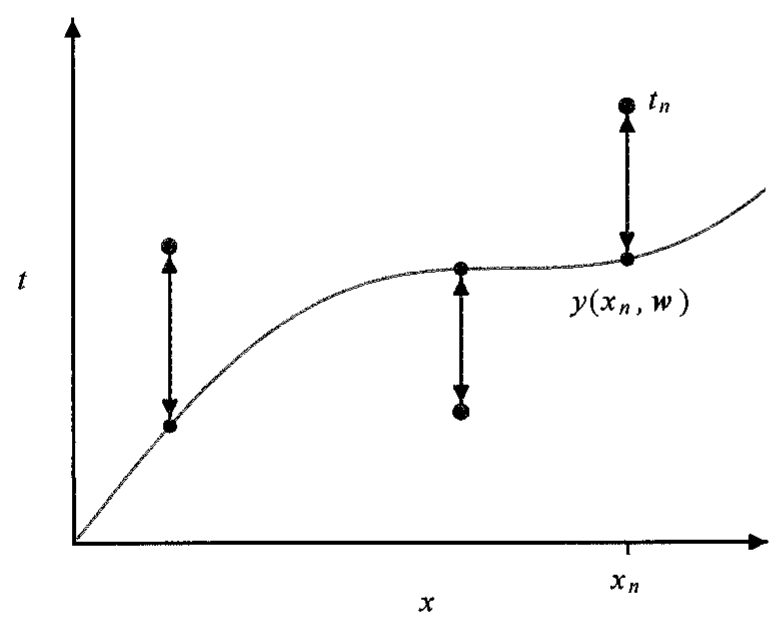
\includegraphics[width=0.5\textwidth]{ch01-fig1-6-sse-geometry.png}
  \caption{平方和误差函数的几何解释［该误差函数对应来自函数 $y(x,\mathbf{w})$ 的每个数据点的位移（如垂直的绿色箭头所示）平方和的一半］}
  \label{figure:ch01-误差函数几何}
\end{figure}

我们可以通过选择能够使 $E(\mathbf{w})$ 尽可能小的 $\mathbf{w}$ 值来解决曲线拟合问题。因为平方和误差函数是系数 $\mathbf{w}$ 的二次函数，其对系数的导数是系数 $\mathbf{w}$ 的线性函数，所以该误差函数的最小化有一个唯一解，记为 $\mathbf{w}^{*}$，可以通过解析形式求得封闭解（也叫解析解）（参见\cref{section:ch04-线性回归}）。

\begin{proposition}[平方和误差函数的最小二乘解]\label{proposition:ch01-最小二乘解}
设 $N,M\in\mathbb{N}$，训练集 $\{(x_n,t_n)\}_{n=1}^{N}\subset\mathbb{R}\times\mathbb{R}$，$\mathbf{t}=(t_1,\cdots,t_N)^{\mathsf{T}}\in\mathbb{R}^{N}$，设计矩阵 $\boldsymbol{\Phi}\in\mathbb{R}^{N\times(M+1)}$ 的第 $n$ 行第 $j$ 列为 $x_n^{\,j}$（$n=1,\cdots,N$，$j=0,\cdots,M$），$E:\mathbb{R}^{M+1}\to[0,\infty)$ 为式\eqref{align:ch01-平方和误差}的平方和误差函数。若 $\boldsymbol{\Phi}$ 列满秩，即 $\operatorname{rank}\boldsymbol{\Phi}=M+1$（此条件蕴含 $N\geqslant M+1$），则
\begin{enumerate}
  \item $\boldsymbol{\Phi}^{\mathsf{T}}\boldsymbol{\Phi}\in\mathbb{R}^{(M+1)\times(M+1)}$ 为对称正定矩阵，因而可逆；
  \item $E$ 在 $\mathbb{R}^{M+1}$ 上的全局极小点存在且唯一，它就是正规方程
  \begin{align*}
    \boldsymbol{\Phi}^{\mathsf{T}}\boldsymbol{\Phi}\mathbf{w}=\boldsymbol{\Phi}^{\mathsf{T}}\mathbf{t}
  \end{align*}
  的唯一解
  \begin{align*}
    \mathbf{w}^{*} = \left(\boldsymbol{\Phi}^{\mathsf{T}}\boldsymbol{\Phi}\right)^{-1}\boldsymbol{\Phi}^{\mathsf{T}}\mathbf{t};
  \end{align*}
  \item 对一切 $\mathbf{w}\in\mathbb{R}^{M+1}$ 有 $E(\mathbf{w})\geqslant E(\mathbf{w}^{*})$，且等号成立当且仅当 $\mathbf{w}=\mathbf{w}^{*}$，故 $E(\mathbf{w}^{*})$ 是 $E$ 在 $\mathbb{R}^{M+1}$ 上的最小值。
\end{enumerate}
\end{proposition}

\begin{proof}
由式\eqref{align:ch01-多项式模型}，对每个 $n\in\{1,\cdots,N\}$ 有 $y(x_n,\mathbf{w})=\sum_{j=0}^{M}w_jx_n^{\,j}=(\boldsymbol{\Phi}\mathbf{w})_n$，故式\eqref{align:ch01-平方和误差}可写成
\begin{align*}
 E(\mathbf{w}) = \frac{1}{2}\left\|\boldsymbol{\Phi}\mathbf{w}-\mathbf{t}\right\|^{2}
 = \frac{1}{2}\left(\mathbf{w}^{\mathsf{T}}\boldsymbol{\Phi}^{\mathsf{T}}\boldsymbol{\Phi}\mathbf{w}
 - 2\,\mathbf{w}^{\mathsf{T}}\boldsymbol{\Phi}^{\mathsf{T}}\mathbf{t}
 + \mathbf{t}^{\mathsf{T}}\mathbf{t}\right),
\end{align*}
由此得梯度与 Hessian 矩阵
\begin{align*}
 \nabla E(\mathbf{w}) = \boldsymbol{\Phi}^{\mathsf{T}}\boldsymbol{\Phi}\mathbf{w} - \boldsymbol{\Phi}^{\mathsf{T}}\mathbf{t},
 \qquad
 \nabla^{2} E(\mathbf{w}) = \boldsymbol{\Phi}^{\mathsf{T}}\boldsymbol{\Phi}.
\end{align*}
对任意 $\mathbf{v}\in\mathbb{R}^{M+1}\setminus\{\mathbf{0}\}$，由 $\boldsymbol{\Phi}$ 列满秩得 $\boldsymbol{\Phi}\mathbf{v}\neq\mathbf{0}$，从而
\begin{align*}
 \mathbf{v}^{\mathsf{T}}\boldsymbol{\Phi}^{\mathsf{T}}\boldsymbol{\Phi}\mathbf{v} = \left\|\boldsymbol{\Phi}\mathbf{v}\right\|^{2} > 0,
\end{align*}
故 $\boldsymbol{\Phi}^{\mathsf{T}}\boldsymbol{\Phi}$ 正定，特别地可逆，第一条成立。

由 $\mathbf{w}^{*}=(\boldsymbol{\Phi}^{\mathsf{T}}\boldsymbol{\Phi})^{-1}\boldsymbol{\Phi}^{\mathsf{T}}\mathbf{t}$ 的定义得 $\boldsymbol{\Phi}^{\mathsf{T}}\boldsymbol{\Phi}\mathbf{w}^{*}=\boldsymbol{\Phi}^{\mathsf{T}}\mathbf{t}$，即 $\nabla E(\mathbf{w}^{*})=\mathbf{0}$。若 $\mathbf{w}$ 也满足 $\nabla E(\mathbf{w})=\mathbf{0}$，则 $\boldsymbol{\Phi}^{\mathsf{T}}\boldsymbol{\Phi}(\mathbf{w}-\mathbf{w}^{*})=\mathbf{0}$，左乘 $(\mathbf{w}-\mathbf{w}^{*})^{\mathsf{T}}$ 得 $\left\|\boldsymbol{\Phi}(\mathbf{w}-\mathbf{w}^{*})\right\|^{2}=0$，故 $\boldsymbol{\Phi}(\mathbf{w}-\mathbf{w}^{*})=\mathbf{0}$，再由列满秩得 $\mathbf{w}=\mathbf{w}^{*}$。因此正规方程有唯一解 $\mathbf{w}^{*}$。

对任意 $\mathbf{w}\in\mathbb{R}^{M+1}$，把两个二次型之差展开得
\begin{align*}
 E(\mathbf{w}) - E(\mathbf{w}^{*})
 = \frac{1}{2}\left\|\boldsymbol{\Phi}(\mathbf{w}-\mathbf{w}^{*})\right\|^{2}
 + (\mathbf{w}-\mathbf{w}^{*})^{\mathsf{T}}\bigl(\boldsymbol{\Phi}^{\mathsf{T}}\boldsymbol{\Phi}\mathbf{w}^{*}-\boldsymbol{\Phi}^{\mathsf{T}}\mathbf{t}\bigr)
 = \frac{1}{2}\left\|\boldsymbol{\Phi}(\mathbf{w}-\mathbf{w}^{*})\right\|^{2} \geqslant 0,
\end{align*}
最后一个等号用到 $\boldsymbol{\Phi}^{\mathsf{T}}\boldsymbol{\Phi}\mathbf{w}^{*}=\boldsymbol{\Phi}^{\mathsf{T}}\mathbf{t}$。故 $E(\mathbf{w}^{*})\leqslant E(\mathbf{w})$ 对一切 $\mathbf{w}$ 成立，且等号成立时 $\boldsymbol{\Phi}(\mathbf{w}-\mathbf{w}^{*})=\mathbf{0}$，再由列满秩得 $\mathbf{w}=\mathbf{w}^{*}$；反之 $\mathbf{w}=\mathbf{w}^{*}$ 时等号成立。于是 $\mathbf{w}^{*}$ 是 $E$ 的唯一全局极小点，第三条成立。
\end{proof}

% SUPPLEMENT: parent=proposition:ch01-最小二乘解; kind=motivation; location=紧随其后的 remark
\begin{remark}
“唯一解”这一结论的真正前提是 $\boldsymbol{\Phi}$ 列满秩，而它等价于：$N\geqslant M+1$，且 $x_1,\cdots,x_N$ 中至少有 $M+1$ 个互不相同的取值（否则 $\boldsymbol{\Phi}$ 的列线性相关）。若这一条件不成立（例如 $N<M+1$，或用到的 $x_n$ 取值过少），则正规方程的解构成一个仿射集，最小化问题有无穷多个解，$\mathbf{w}^{*}$ 不再唯一，但 $E$ 的最小值仍然存在。
这解释了本例的一个细节：\cref{subsection:ch01-模型复杂度}中 $M=9$、$N=10$ 恰好处在临界情形 $N=M+1$，自由度正好等于数据点个数，因此可以精确插值；若数据点少于自由度，插值解更多，系数的选取将更加任意，这也是\cref{table:ch01-多项式系数}中 $M=9$ 一列出现巨大系数的原因。
\end{remark}

最终的多项式由函数 $y(x,\mathbf{w}^{*})$ 给出。

\subsection{模型复杂度}\label{subsection:ch01-模型复杂度}

我们还面临选择多项式的阶数 $M$ 的问题，这将引出模型比较（model comparison）或模型选择（model selection）这一重要概念。在\cref{figure:ch01-不同阶数拟合}中，我们展示了 $4$ 个拟合实例，它们分别使用阶数 $M=0,1,3,9$ 的多项式来拟合\cref{figure:ch01-正弦拟合训练集}所示的数据集。

\begin{figure}[htbp]
  \centering
  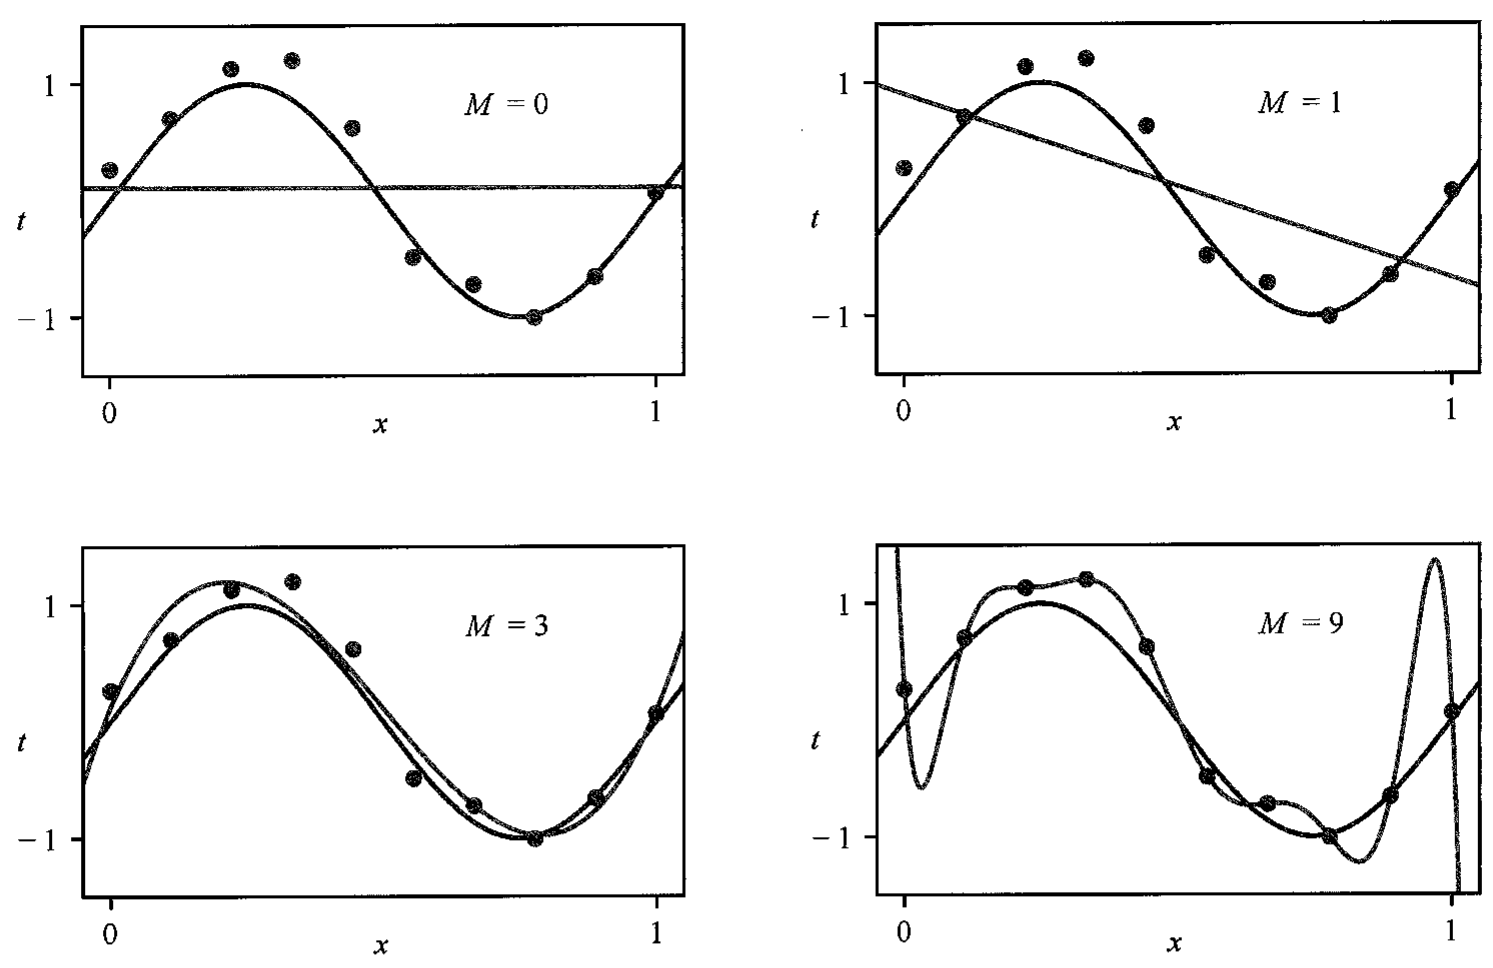
\includegraphics[width=0.92\textwidth]{ch01-fig1-7-poly-fits.png}
  \caption{具有不同阶数的多项式图示。多项式如红色曲线所示。这里通过最小化平方和误差函数（见式\eqref{align:ch01-平方和误差}）来拟合\cref{figure:ch01-正弦拟合训练集}所示的数据集}
  \label{figure:ch01-不同阶数拟合}
\end{figure}

可以发现，常数（$M=0$）和一阶（$M=1$）多项式对数据的拟合较差，因此对函数 $\sin(2\pi x)$ 的表示较差。三阶（$M=3$）多项式似乎对函数 $\sin(2\pi x)$ 给出了最佳拟合。高阶（$M=9$）多项式得到了一个对训练数据完美的拟合。事实上，这个多项式曲线精确地穿过了每一个数据点，使得误差 $E(\mathbf{w}^{*})=0$。然而，拟合出的曲线却出现了剧烈的波动，完全不能反映出函数 $\sin(2\pi x)$ 的真实形态。这种现象称为过拟合（over-fitting）。

\begin{definition}[过拟合]\label{definition:ch01-过拟合}
设 $\{y(\cdot;\mathbf{w}):\mathbf{w}\in\mathcal{W}_{m}\}_{m\in\mathbb{N}}$ 为一族模型，其中复杂度指标 $m$ 取正整数，参数空间 $\mathcal{W}_{m}\subseteq\mathbb{R}^{P_{m}}$；设训练集 $\mathcal{D}_{\mathrm{tr}}$ 与测试集 $\mathcal{D}_{\mathrm{te}}$ 为来自同一分布的独立样本，损失函数 $\ell:\mathcal{Y}\times\mathcal{Y}\to[0,\infty)$。记 $\mathbf{w}_{m}\in\mathcal{W}_{m}$ 为训练误差的一个极小点，即
\begin{align*}
  \mathbf{w}_{m}\in\arg\min_{\mathbf{w}\in\mathcal{W}_{m}}\frac{1}{\lvert\mathcal{D}_{\mathrm{tr}}\rvert}\sum_{(x,t)\in\mathcal{D}_{\mathrm{tr}}}\ell\bigl(y(x;\mathbf{w}),t\bigr),
\end{align*}
并记 $\mathbf{w}_{m}$ 在训练集与测试集上的平均损失分别为 $\widehat{R}_{\mathrm{tr}}(m)$ 与 $\widehat{R}_{\mathrm{te}}(m)$。若存在 $m_{1}<m_{2}$ 使得
\begin{enumerate}
  \item $\widehat{R}_{\mathrm{tr}}(m_{2})\leqslant\widehat{R}_{\mathrm{tr}}(m_{1})$，即训练误差不随复杂度增加而上升；
  \item $\widehat{R}_{\mathrm{te}}(m_{2})>\widehat{R}_{\mathrm{te}}(m_{1})$，即测试误差随复杂度增加而上升，
\end{enumerate}
则这一现象称为\textbf{过拟合}（over-fitting），并称复杂度 $m_{2}$ 处的模型相对 $m_{1}$ \textbf{过拟合}了训练数据。
\end{definition}

% SUPPLEMENT: parent=definition:ch01-过拟合; kind=motivation; location=紧随其后的 remark
\begin{remark}
过拟合的实质是模型把训练数据中的\textbf{随机噪声}也当作规律学习了。$M=9$ 的多项式有 $10$ 个可调系数，而训练点恰有 $10$ 个，于是它可以用一条剧烈振荡的曲线精确穿过每一点（$E(\mathbf{w}^{*})=0$），而这条曲线在数据点之间、尤其是在区间两端完全偏离 $\sin(2\pi x)$。
条件是相对于数据量而言的：同样的 $M=9$，在 $N=15$ 或 $N=100$ 时过拟合就明显减弱（\cref{figure:ch01-数据集大小}）。因此“参数多必然过拟合”是不对的，正确的说法是“参数相对于数据量过多时容易过拟合”；\cref{subsection:ch01-正则化}将说明如何在参数数量不变的前提下抑制这一现象，而深度学习还会出现参数远超样本数却泛化良好的情形（参见\cref{subsection:ch09-双重下降}）。
\end{remark}

我们的目标是让模型获得良好的泛化能力，使其能够对新的数据做出准确的预测。为了定量地探究泛化性能与模型复杂度 $M$ 之间的依赖关系，我们可以引入一个独立的测试集。该测试集包含 $100$ 个数据点，其生成方式与训练集相同。针对每一个 $M$ 值，我们不仅可以计算出模型在训练集上的残差 $E(\mathbf{w}^{*})$（式\eqref{align:ch01-平方和误差}），还可以计算出其在测试集上的残差 $E(\mathbf{w}^{*})$。与评估误差函数 $E(\mathbf{w})$ 相比，有时使用均方根（Root Mean Square, RMS）误差更为方便，均方根误差定义如下：

\begin{definition}[均方根误差]\label{definition:ch01-均方根误差}
设 $N\in\mathbb{N}$，数据集 $\{(x_n,t_n)\}_{n=1}^{N}\subset\mathbb{R}\times\mathbb{R}$，模型 $y(\cdot,\mathbf{w}):\mathbb{R}\to\mathbb{R}$ 的参数为 $\mathbf{w}\in\mathbb{R}^{M+1}$，$E(\mathbf{w})$ 为式\eqref{align:ch01-平方和误差}的平方和误差函数。由
\begin{align}
  E_{\mathrm{RMS}} = \sqrt{\frac{1}{N} \sum_{n=1}^{N} \left\{ y(x_n, \mathbf{w}) - t_n \right\}^2}
  \label{align:ch01-RMS误差}
\end{align}
定义的量称为该数据集上的\textbf{均方根误差}（Root Mean Square error）。其中求和范围为 $n=1,\cdots,N$，$x_n$ 为输入、$t_n$ 为目标值；$E_{\mathrm{RMS}}$ 与目标变量同量纲，且 $E_{\mathrm{RMS}}=\sqrt{2E(\mathbf{w})/N}$。
\end{definition}

% SUPPLEMENT: parent=definition:ch01-均方根误差; kind=motivation; location=紧随其后的 remark
\begin{remark}
两个修正各有明确目的：除以 $N$ 使不同大小的数据集可以在同一基准下比较（否则误差和会随 $N$ 增大而增大，训练集与测试集的数值不可比）；开平方使 $E_{\mathrm{RMS}}$ 与目标变量 $t$ 具有相同的量纲，因而数值可以被直接解读为“平均偏差多少个单位”。
需要强调，$E_{\mathrm{RMS}}$ 与 $E$ 只差一个由 $N$ 决定的单调变换，故对同一数据集而言两者的极小点相同；改变的是\textbf{可读性}与\textbf{可比性}，不是最优解。\cref{figure:ch01-均方根误差曲线}与\cref{figure:ch01-正则化参数影响}中的纵轴都用 $E_{\mathrm{RMS}}$，正是为了把训练集与测试集放在同一把尺子上比较。
\end{remark}

公式中的 $1/N$ 是为了让不同大小的数据集能够在相同的基准下进行比较，而求平方根则是为了确保 $E_{\mathrm{RMS}}$ 是在与目标变量 $t$ 相同的尺度上（以相同的单位）进行测量的。\cref{figure:ch01-均方根误差曲线}展示了不同 $M$ 值的训练集和测试集的 RMS 误差图。测试集上的 RMS 误差反映了我们根据新观测数据 $x$ 预测其对应 $t$ 值的能力。

\begin{figure}[htbp]
  \centering
  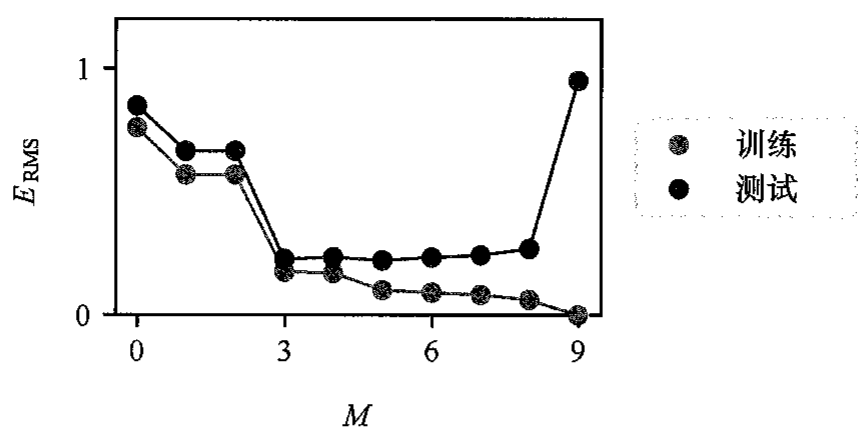
\includegraphics[width=0.62\textwidth]{ch01-fig1-8-rms-vs-m.png}
  \caption{由式\eqref{align:ch01-RMS误差}定义的均方根误差图（在训练集和独立的测试集上对 $M$ 的各个值进行评估）}
  \label{figure:ch01-均方根误差曲线}
\end{figure}

从\cref{figure:ch01-均方根误差曲线}中可以看出，当 $M$ 值较小时测试集误差较大，这是因为此时的多项式模型灵活性不足，无法捕捉函数 $\sin(2\pi x)$ 中的振荡。当 $M$ 取值在 $[3,8]$ 时，测试集误差较小，同时这些模型也能合理地表示出数据的生成函数 $\sin(2\pi x)$，如\cref{figure:ch01-不同阶数拟合}中 $M=3$ 时所示。

当 $M=9$ 时，训练集误差变为零。这是符合预期的，因为该多项式包含 $10$ 个自由度（对应 $10$ 个系数 $w_0,\cdots,w_9$），所以可以精确地调整到训练集中的 $10$ 个数据点。然而，如\cref{figure:ch01-不同阶数拟合}和\cref{figure:ch01-均方根误差曲线}所示，测试集误差变得极大，函数 $y(x,\mathbf{w}^{*})$ 表现出剧烈振荡。

这可能看起来很矛盾，因为一个给定阶数的多项式包含了所有更低阶的多项式作为特例。因此，$M=9$ 的多项式理应能够产生至少与 $M=3$ 的多项式一样好的结果。此外，我们或许会认为，预测新数据的最佳模型就应该是生成这些数据的真实函数 $\sin(2\pi x)$ 本身（我们后续将验证这一点）。同时，我们知道 $\sin(2\pi x)$ 的幂级数展开式中包含了所有阶数的项，所以我们会很自然地推断，随着模型复杂度 $M$ 的增加，预测效果应该会持续提升。

\begin{proposition}[训练误差随阶数单调不增]\label{proposition:ch01-训练误差单调性}
设 $N\in\mathbb{N}$，训练集 $\{(x_n,t_n)\}_{n=1}^{N}\subset\mathbb{R}\times\mathbb{R}$；对每个 $M\in\mathbb{N}$，设 $E_{M}:\mathbb{R}^{M+1}\to[0,\infty)$ 为 $M$ 阶多项式模型的平方和误差函数（式\eqref{align:ch01-平方和误差}），并记
\begin{align*}
  E_{M}^{*}=\inf_{\mathbf{w}\in\mathbb{R}^{M+1}}E_{M}(\mathbf{w}).
\end{align*}
则对每个 $M$ 有 $E_{M}^{*}\in[0,\infty)$，且
\begin{align*}
  E_{0}^{*} \geqslant E_{1}^{*} \geqslant E_{2}^{*} \geqslant \cdots,
\end{align*}
即最小训练误差（下确界）随阶数单调不增。特别地，$E_{9}^{*}\leqslant E_{3}^{*}$。
\end{proposition}

\begin{proof}
对每个 $M$，由 $E_{M}(\mathbf{w})\geqslant0$ 得 $E_{M}^{*}\geqslant0$；又 $E_{M}(\mathbf{0})=\frac{1}{2}\sum_{n=1}^{N}t_n^{2}<\infty$，故 $E_{M}^{*}<\infty$，于是 $E_{M}^{*}\in[0,\infty)$。

设 $M<M'$。对任意 $\mathbf{w}=(w_0,\cdots,w_M)\in\mathbb{R}^{M+1}$，令 $\tilde{\mathbf{w}}=(w_0,\cdots,w_M,0,\cdots,0)\in\mathbb{R}^{M'+1}$，则对一切 $x\in\mathbb{R}$ 有
\begin{align*}
 \sum_{j=0}^{M'} \tilde{w}_j x^{j} = \sum_{j=0}^{M} w_j x^{j},
\end{align*}
即两个系数向量给出同一个多项式函数，故在 $x_1,\cdots,x_N$ 上给出同一组预测值，从而 $E_{M'}(\tilde{\mathbf{w}})=E_{M}(\mathbf{w})$。于是
\begin{align*}
 \left\{E_{M}(\mathbf{w}) : \mathbf{w}\in\mathbb{R}^{M+1}\right\} \subseteq \left\{E_{M'}(\mathbf{w}) : \mathbf{w}\in\mathbb{R}^{M'+1}\right\}.
\end{align*}
对任意 $\mathbf{w}\in\mathbb{R}^{M+1}$，由下确界的定义有 $E_{M'}^{*}\leqslant E_{M'}(\tilde{\mathbf{w}})=E_{M}(\mathbf{w})$；对 $\mathbf{w}$ 取下确界得 $E_{M'}^{*}\leqslant E_{M}^{*}$。由 $M<M'$ 的任意性得序列单调不增；取 $M=3$、$M'=9$ 得 $E_{9}^{*}\leqslant E_{3}^{*}$。
\end{proof}

% SUPPLEMENT: parent=proposition:ch01-训练误差单调性; kind=motivation; location=紧随其后的 remark
\begin{remark}
这条命题澄清了表面矛盾的确切含义：$M$ 增大只会让\textbf{训练}误差不变或下降，绝不会使它上升；因此\cref{figure:ch01-均方根误差曲线}中 $M=9$ 时测试误差的剧烈上升，只能来自泛化行为的恶化，而不是训练集拟合能力的退步。换言之，“高阶模型更灵活”与“高阶模型泛化更差”并不冲突——灵活性保证它能把训练误差压得更低，也正因为如此它更容易把噪声一起拟合进去。
条件的边界同样重要：命题只比较训练误差，并未断言测试误差也单调；它也不要求解唯一（$N<M+1$ 时\cref{proposition:ch01-最小二乘解}的唯一性条件失效，但下确界仍存在，命题的证明只用到了函数族的包含关系）。
\end{remark}

通过观察\cref{table:ch01-多项式系数}中不同阶数多项式拟合得到的系数 $\mathbf{w}^{*}$，我们可以更深入地了解这个问题。

\begin{table}[htbp]
  \centering
  \caption{不同阶数多项式的系数 $\mathbf{w}^{*}$。注意观察随着多项式阶数的增加，系数的变化幅度是如何急剧增大的}
  \label{table:ch01-多项式系数}
  \begin{tabular}{c *{4}{r}}
    \toprule
     & $M=0$ & $M=1$ & $M=3$ & $M=9$ \\
    \midrule
    $w_0^{*}$ & $0.11$ & $0.90$ & $0.12$ & $0.26$ \\
    $w_1^{*}$ &  & $-1.58$ & $11.20$ & $-66.13$ \\
    $w_2^{*}$ &  &  & $-33.67$ & $1{,}665.69$ \\
    $w_3^{*}$ &  &  & $-22.43$ & $-15{,}566.61$ \\
    $w_4^{*}$ &  &  &  & $76{,}321.23$ \\
    $w_5^{*}$ &  &  &  & $-217{,}389.15$ \\
    $w_6^{*}$ &  &  &  & $370{,}626.48$ \\
    $w_7^{*}$ &  &  &  & $-372{,}051.47$ \\
    $w_8^{*}$ &  &  &  & $202{,}540.70$ \\
    $w_9^{*}$ &  &  &  & $-46{,}080.94$ \\
    \bottomrule
  \end{tabular}
\end{table}

我们注意到，随着 $M$ 的增加，系数的幅度越来越大。特别是当 $M=9$ 时，为了让对应的多项式曲线能精准地穿过每一个数据点，这些系数被精细地调整到了很大的正值或负值。但在数据点之间，尤其是在数据范围的两端附近，曲线却出现了大幅度的摆动，正如我们在\cref{figure:ch01-不同阶数拟合}中看到的那样。直观地看，当多项式模型具有较大的 $M$ 值时，它变得更加灵活，从而更容易受到目标值上随机噪声的影响，并过度拟合了这些噪声。

为进一步探究该现象，我们观察随着数据集大小的变化，模型学习效果的相应变化，如\cref{figure:ch01-数据集大小}所示。可以看出，当模型复杂度固定时，数据集越大，过拟合现象就越不明显。换言之，数据量越大，我们就能用越复杂（即更灵活）的模型去拟合数据。

经典统计学中有一条常用的启发式经验：训练数据点的数量应至少是模型中可学习参数数量的若干倍（比如 $5$ 倍或 $10$ 倍）。然而，我们在本书继续探讨深度学习后会发现，即使模型参数的数量远远超过训练数据点的数量，也一样可以获得非常出色的结果（参见\cref{subsection:ch09-双重下降}）。

\begin{figure}[htbp]
  \centering
  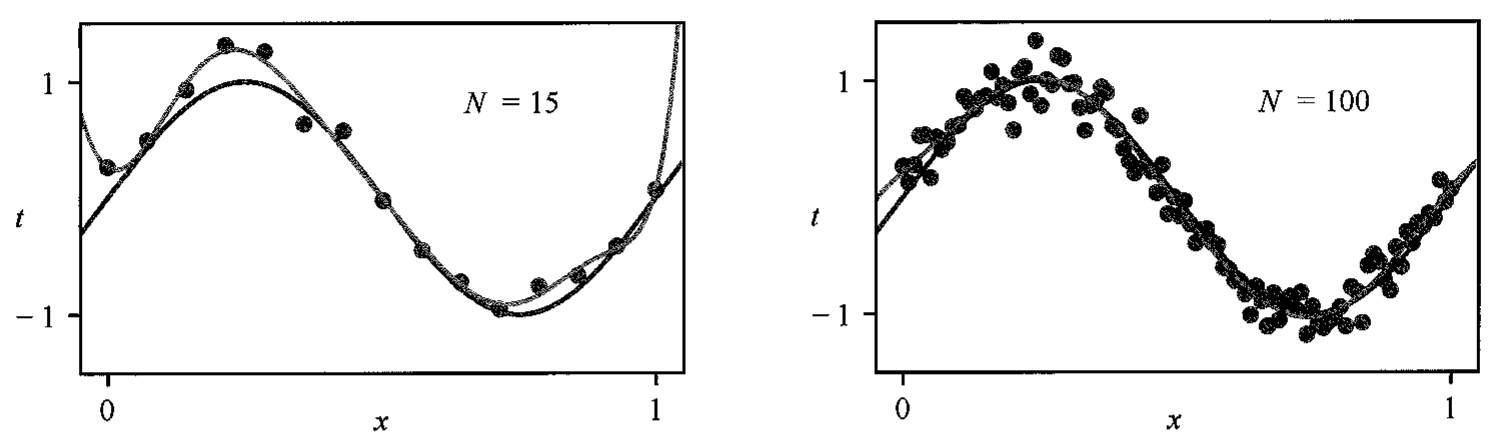
\includegraphics[width=0.95\textwidth]{ch01-fig1-9-dataset-size.png}
  \caption{使用 $M=9$ 的多项式最小化平方和误差函数所获得的解决方案（左图为拟合 $N=15$ 个数据点所获得的解，右图为拟合 $N=100$ 个数据点所获得的解。可以看到，大的数据集可以减少过拟合）}
  \label{figure:ch01-数据集大小}
\end{figure}

\subsection{正则化}\label{subsection:ch01-正则化}

根据可用训练集的大小来限制模型中参数的数量，其结果有些不尽如人意。而根据待解决问题的复杂性来选择模型的复杂性似乎更合理。作为限制参数数量的替代方案，正则化（regularization）技术经常被用于控制过拟合现象，它通过向误差函数添加一个惩罚项来抑制系数取值过大。最简单的惩罚项采用所有系数的平方和的形式，误差函数变为

\begin{definition}[正则化]\label{definition:ch01-正则化}
设 $N,M\in\mathbb{N}$，训练集 $\{(x_n,t_n)\}_{n=1}^{N}\subset\mathbb{R}\times\mathbb{R}$，$M$ 阶多项式模型 $y(\cdot,\mathbf{w}):\mathbb{R}\to\mathbb{R}$ 由式\eqref{align:ch01-多项式模型}给出，$\mathbf{w}=(w_0,\cdots,w_M)\in\mathbb{R}^{M+1}$，$\lambda\geqslant0$ 为给定常数，$\mathcal{J}\subseteq\{0,1,\cdots,M\}$ 为被惩罚的指标集。在目标函数中加入惩罚项以抑制系数幅度的做法称为\textbf{正则化}（regularization），$\lambda$ 称为\textbf{正则化系数}。当 $\mathcal{J}=\{0,1,\cdots,M\}$ 时，由
\begin{align}
  \tilde{E}(\mathbf{w}) = \frac{1}{2} \sum_{n=1}^{N} \left\{ y(x_n, \mathbf{w}) - t_n \right\}^2 + \frac{\lambda}{2} \sum_{j=0}^{M} w_j^2
  \label{align:ch01-正则化误差}
\end{align}
定义的 $\tilde{E}:\mathbb{R}^{M+1}\to[0,\infty)$ 称为\textbf{正则化误差函数}（regularized error function）。其中 $\|\mathbf{w}\|^{2}=\mathbf{w}^{\mathsf{T}}\mathbf{w}=\sum_{j=0}^{M}w_j^{2}$，$\lambda$ 控制惩罚项与平方和误差项的相对权重；一般地，惩罚项取 $\frac{\lambda}{2}\sum_{j\in\mathcal{J}}w_j^{2}$，本书通常取 $\mathcal{J}=\{1,\cdots,M\}$，即不惩罚 $w_0$。
\end{definition}

% SUPPLEMENT: parent=definition:ch01-正则化; kind=motivation; location=紧随其后的 remark
\begin{remark}
动机是给“系数变大”本身标价：既然过拟合表现为系数被调整到很大的正负值（\cref{table:ch01-多项式系数}），就在目标函数中直接惩罚系数的幅度，使模型在拟合数据与保持系数较小之间折中。$\lambda$ 是这一折中的价格：$\lambda=0$ 时，式\eqref{align:ch01-正则化误差}退化为式\eqref{align:ch01-平方和误差}；$\lambda$ 增大时系数被压向零，模型的有效复杂度下降。
条件上有两点容易忽略。其一，惩罚项通常\textbf{不含} $w_0$：若惩罚 $w_0$，则结果会依赖目标变量原点如何选取——把 $t$ 整体平移一个常数，本应只改变 $w_0$ 而不改变曲线形状，惩罚 $w_0$ 却会使最优解随平移而变。当然也可以惩罚 $w_0$，但须为它单独配置系数（参见\cref{section:ch09-权重衰减}）。其二，要求 $\lambda\geqslant 0$：若允许 $\lambda<0$，惩罚项变成奖励项，问题可能无下界。
\end{remark}

注意，正则化项中通常不包含系数 $w_0$，因为如果包含 $w_0$，就会导致最终结果受到目标变量所选原点的影响（Hastie, Tibshirani, and Friedman, 2009）。当然也可以包含 $w_0$，但需要单独为其配置一个正则化系数（参见\cref{section:ch09-权重衰减}）。同样，我们可以求得式\eqref{align:ch01-正则化误差}中误差函数的精确闭式解（见\cref{exercise:ch04-02}）。在统计学文献中，这类方法被称为收缩方法（shrinkage），因为它们会使系数的值缩小。在神经网络领域，这种方法称为权重衰减（weight decay），因为神经网络中的参数通常称为权重，而这种正则化手段会促使这些权重向零衰减。

\cref{figure:ch01-正则化拟合}展示了采用正则化误差函数（式\eqref{align:ch01-正则化误差}）对 $9$ 阶（$M=9$）多项式进行拟合的结果，所用数据集与之前相同。观察发现，当取 $\ln\lambda=-18$ 时，过拟合现象被有效抑制，此时的拟合曲线与目标函数 $\sin(2\pi x)$ 相当接近。反之，若 $\lambda$ 取值过大，则会导致欠拟合，如\cref{figure:ch01-正则化拟合}中 $\ln\lambda=0$ 的情形。

\begin{figure}[htbp]
  \centering
  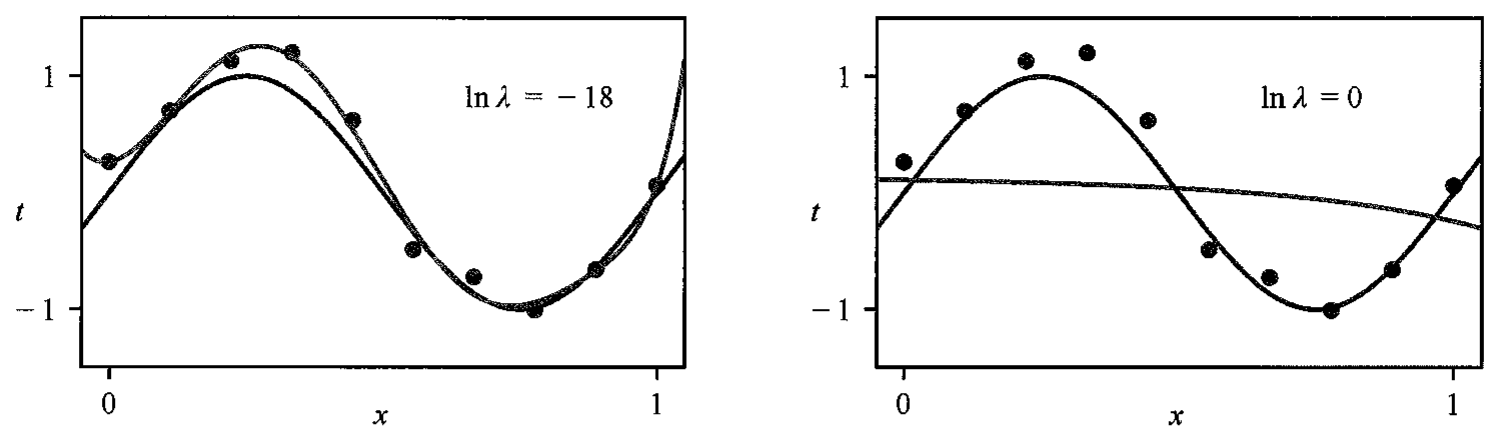
\includegraphics[width=0.95\textwidth]{ch01-fig1-10-regularized-fits.png}
  \caption{使用正则化误差函数［式\eqref{align:ch01-正则化误差}］对\cref{figure:ch01-正弦拟合训练集}中数据集进行拟合所得的 $M=9$ 阶多项式的曲线。其中正则化参数 $\lambda$ 取两个值，分别对应于 $\ln\lambda=-\infty$ 和 $\ln\lambda=0$。无正则化项的情况，即 $\lambda=0$（对应 $\ln\lambda=-\infty$）的情况，显示在\cref{figure:ch01-不同阶数拟合}的右下图中}
  \label{figure:ch01-正则化拟合}
\end{figure}

\cref{table:ch01-正则化系数}给出了不同 $\lambda$ 值下拟合得到的多项式系数，这些数值表明，正则化确实发挥了预期作用，有效减小了系数的幅度。

\begin{table}[htbp]
  \centering
  \caption{正则化参数 $\lambda$ 取不同值时，$M=9$ 的多项式模型的系数 $\mathbf{w}^{*}$。注意，$\ln\lambda=-\infty$ 对应未采用正则化的模型，也就是\cref{figure:ch01-不同阶数拟合}右下图中的拟合结果。可见，随着 $\lambda$ 值的增大，系数的量级会减小}
  \label{table:ch01-正则化系数}
  \begin{tabular}{c *{3}{r}}
    \toprule
     & $\ln\lambda=-\infty$ & $\ln\lambda=-18$ & $\ln\lambda=0$ \\
    \midrule
    $w_0^{*}$ & $0.26$ & $0.26$ & $0.11$ \\
    $w_1^{*}$ & $-66.13$ & $0.64$ & $-0.07$ \\
    $w_2^{*}$ & $1{,}665.69$ & $43.68$ & $-0.09$ \\
    $w_3^{*}$ & $-15{,}566.61$ & $-144.00$ & $-0.07$ \\
    $w_4^{*}$ & $76{,}321.23$ & $57.90$ & $-0.05$ \\
    $w_5^{*}$ & $-217{,}389.15$ & $117.36$ & $-0.04$ \\
    $w_6^{*}$ & $370{,}626.48$ & $9.87$ & $-0.02$ \\
    $w_7^{*}$ & $-372{,}051.47$ & $-90.02$ & $-0.01$ \\
    $w_8^{*}$ & $202{,}540.70$ & $-70.90$ & $-0.01$ \\
    $w_9^{*}$ & $-46{,}080.94$ & $75.26$ & $0.00$ \\
    \bottomrule
  \end{tabular}
\end{table}

通过绘制训练集和测试集的 RMS 误差（式\eqref{align:ch01-RMS误差}）与 $\ln\lambda$ 的关系，可以看出正则化项对泛化误差的影响，如\cref{figure:ch01-正则化参数影响}所示。可以看到，$\lambda$ 现在控制了模型的有效复杂性，从而决定了过拟合的程度。

\begin{figure}[htbp]
  \centering
  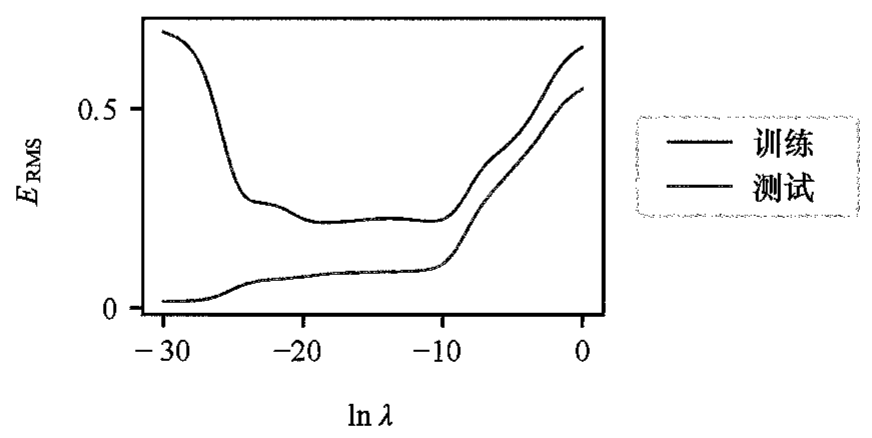
\includegraphics[width=0.62\textwidth]{ch01-fig1-11-rms-vs-lambda.png}
  \caption{$M=9$ 的多项式的 RMS 误差与 $\ln\lambda$ 的关系}
  \label{figure:ch01-正则化参数影响}
\end{figure}

\subsection{模型选择}\label{subsection:ch01-模型选择}

在本例中，$\lambda$ 作为一个超参数（hyperparameter），它的值在基于误差函数最小化来确定模型参数 $\mathbf{w}$ 的过程中始终保持不变。

\begin{definition}[超参数]\label{definition:ch01-超参数}
设训练集 $\mathcal{D}$，参数空间 $\mathcal{W}\subseteq\mathbb{R}^{P}$（$P\in\mathbb{N}$），误差函数 $E:\mathcal{W}\to[0,\infty)$，参数 $\mathbf{w}$ 由求解 $\min_{\mathbf{w}\in\mathcal{W}}E(\mathbf{w})$ 确定。设 $\eta$ 为某个取值可在该极小化之前指定的量（如正则化系数 $\lambda$、多项式阶数 $M$），$\Theta_{\eta}$ 为它的取值集合，且 $\mathcal{W}$ 与 $E$ 依赖于 $\eta$，即 $E(\cdot;\eta):\mathcal{W}_{\eta}\to[0,\infty)$。若对每个 $\eta\in\Theta_{\eta}$，$\eta$ 的取值都在求解 $\min_{\mathbf{w}\in\mathcal{W}_{\eta}}E(\mathbf{w};\eta)$ 之前固定，并在该求解过程中保持不变、不作为极小化的变量，则 $\eta$ 称为该学习问题的\textbf{超参数}（hyperparameter），$\Theta_{\eta}$ 称为它的\textbf{超参数空间}。
\end{definition}

% SUPPLEMENT: parent=definition:ch01-超参数; kind=motivation; location=紧随其后的 remark
\begin{remark}
区分参数与超参数的标准是“由谁的最小化决定”，而不是“是否可以被学习”：$\mathbf{w}$ 由最小化 $E$ 或 $\tilde{E}$ 得到，$\lambda$ 与阶数 $M$ 则必须在优化之前就选定，随后在整个训练过程中保持不变。
这一安排的必要性来自下一段：若把 $\lambda$ 也交给同一个最小化过程，它会被推向 $0$（\cref{proposition:ch01-超参数不可联合优化}），正则化随即失效。因此超参数的合理取值只能借助\textbf{另一个}判据来确定，例如在一份独立的验证数据上的误差，这正是后面引入验证集与交叉验证的原因。
\end{remark}

需要注意的是，我们不能通过同时对 $\mathbf{w}$ 和 $\lambda$ 最小化误差函数的方式来简单地确定 $\lambda$ 的取值，因为这样会导致 $\lambda$ 趋近于 $0$，从而产生一个在训练集上误差极小甚至为零的过拟合模型。

\begin{proposition}[正则化系数不能与参数联合优化]\label{proposition:ch01-超参数不可联合优化}
设 $N,M\in\mathbb{N}$，训练集 $\{(x_n,t_n)\}_{n=1}^{N}\subset\mathbb{R}\times\mathbb{R}$，$E:\mathbb{R}^{M+1}\to[0,\infty)$ 与 $\tilde{E}:\mathbb{R}^{M+1}\times[0,\infty)\to[0,\infty)$ 分别为式\eqref{align:ch01-平方和误差}与式\eqref{align:ch01-正则化误差}的平方和误差函数与正则化误差函数。则
\begin{align*}
  \inf_{\mathbf{w}\in\mathbb{R}^{M+1}}\ \inf_{\lambda\geqslant 0}\tilde{E}(\mathbf{w},\lambda)
  = \inf_{\mathbf{w}\in\mathbb{R}^{M+1}}E(\mathbf{w}),
\end{align*}
且对每个 $\mathbf{w}\in\mathbb{R}^{M+1}\setminus\{\mathbf{0}\}$ 与每个 $\lambda>0$ 有 $\tilde{E}(\mathbf{w},\lambda)>\tilde{E}(\mathbf{w},0)=E(\mathbf{w})$；因此若 $\mathbf{w}\neq\mathbf{0}$ 使 $\tilde{E}(\mathbf{w},\cdot)$ 在 $[0,\infty)$ 上取到最小值，则该最小值只能在 $\lambda=0$ 处取到。
\end{proposition}

\begin{proof}
由式\eqref{align:ch01-正则化误差}，
\begin{align*}
 \tilde{E}(\mathbf{w},\lambda)=E(\mathbf{w})+\frac{\lambda}{2}\left\|\mathbf{w}\right\|^{2},
 \qquad (\mathbf{w},\lambda)\in\mathbb{R}^{M+1}\times[0,\infty).
\end{align*}
对固定的 $\mathbf{w}$，上式右端作为 $\lambda$ 的函数是仿射函数，斜率为 $\frac{1}{2}\|\mathbf{w}\|^{2}\geqslant0$。若 $\mathbf{w}=\mathbf{0}$，则 $\tilde{E}(\mathbf{w},\lambda)=E(\mathbf{w})$ 对一切 $\lambda\geqslant0$ 成立，故 $\inf_{\lambda\geqslant0}\tilde{E}(\mathbf{w},\lambda)=E(\mathbf{w})$ 在 $\lambda=0$ 处取到。若 $\mathbf{w}\neq\mathbf{0}$，则斜率严格为正，$\tilde{E}(\mathbf{w},\cdot)$ 在 $[0,\infty)$ 上严格递增，故 $\tilde{E}(\mathbf{w},\lambda)\geqslant\tilde{E}(\mathbf{w},0)=E(\mathbf{w})$，且 $\lambda>0$ 时不等号严格成立。于是对每个 $\mathbf{w}\in\mathbb{R}^{M+1}$ 有
\begin{align*}
 \inf_{\lambda\geqslant 0}\tilde{E}(\mathbf{w},\lambda)=\tilde{E}(\mathbf{w},0)=E(\mathbf{w}),
\end{align*}
且当 $\mathbf{w}\neq\mathbf{0}$ 时这个下确界只在 $\lambda=0$ 处取到。对 $\mathbf{w}$ 取下确界得
\begin{align*}
 \inf_{\mathbf{w}\in\mathbb{R}^{M+1}}\ \inf_{\lambda\geqslant 0}\tilde{E}(\mathbf{w},\lambda)
 =\inf_{\mathbf{w}\in\mathbb{R}^{M+1}}E(\mathbf{w}).
\end{align*}
若 $\mathbf{w}\neq\mathbf{0}$ 使 $\tilde{E}(\mathbf{w},\cdot)$ 在 $[0,\infty)$ 上取到最小值，则由上述严格递增性，该最小值点满足 $\lambda=0$。
\end{proof}

% SUPPLEMENT: parent=proposition:ch01-超参数不可联合优化; kind=motivation; location=紧随其后的 remark
\begin{remark}
结论与原书的表述“$\lambda$ 会趋近于 $0$”一致，但这里的论证更彻底：不是“趋近”，而是在无约束的联合优化下最优值\textbf{恰为} $0$——惩罚项只会增加目标函数值，任何正的 $\lambda$ 都不如 $\lambda=0$ 划算。这解释了为什么正则化系数必须被排除在训练目标之外。
条件方面，论证只用到 $\|\mathbf{w}\|^{2}\geqslant 0$ 与 $\tilde{E}$ 关于 $\lambda$ 的单调性；若把 $\lambda$ 限制在一个正的区间并另加约束，结论会改变，但那样的约束已不属于“最小化误差函数”本身。同理，阶数 $M$ 也不能与 $\mathbf{w}$ 联合优化：由于 $E_{M}^{*}$ 随 $M$ 单调不增（\cref{proposition:ch01-训练误差单调性}），联合优化必然选出最大的 $M$。
\end{remark}

类似地，多项式的阶数 $M$ 也是模型的一个超参数，单纯地优化训练集误差关于 $M$ 的取值会导致 $M$ 过大，同样会引发过拟合问题。因此，我们需要找到一种有效的方法来确定这些超参数的合理取值。\cref{section:ch01-深度学习的影响}的讲述提供了一种简单的思路，即将已有的数据集划分为训练集和验证集（validation set）［也称为保留集（hold-out set）或开发集（development set）］，其中训练集用于确定模型系数 $\mathbf{w}$，而我们最终选择在验证集上误差最小的模型。如果使用有限规模的数据集多次迭代模型设计，也可能会出现对验证集的过拟合现象。为此，通常需要预留出测试集，用于对最终选定模型的性能进行评估。

\begin{definition}[验证集与测试集]\label{definition:ch01-验证集与测试集}
设数据集 $\mathcal{D}$ 由 $N\in\mathbb{N}$ 个样本组成，并划分为三个互不相交的子集：
\begin{align*}
  \mathcal{D}=\mathcal{D}_{\mathrm{tr}}\cup\mathcal{D}_{\mathrm{val}}\cup\mathcal{D}_{\mathrm{te}},\qquad
  \mathcal{D}_{\mathrm{tr}}\cap\mathcal{D}_{\mathrm{val}}=\mathcal{D}_{\mathrm{tr}}\cap\mathcal{D}_{\mathrm{te}}=\mathcal{D}_{\mathrm{val}}\cap\mathcal{D}_{\mathrm{te}}=\varnothing .
\end{align*}
\begin{enumerate}
  \item 若 $\mathcal{D}_{\mathrm{tr}}$ 只用于确定模型参数 $\mathbf{w}$，则它称为\textbf{训练集}（training set）；
  \item 若 $\mathcal{D}_{\mathrm{val}}$ 不参与 $\mathbf{w}$ 的确定，而用于在若干候选模型或候选超参数设置中选出在其上平均损失最小的一个，则它称为\textbf{验证集}（validation set），也称为\textbf{保留集}（hold-out set）或\textbf{开发集}（development set）；
  \item 若 $\mathcal{D}_{\mathrm{te}}$ 在模型与超参数选定之前不被使用，只用于评估最终选定的模型，则它称为\textbf{测试集}（test set）。
\end{enumerate}
\end{definition}

% SUPPLEMENT: parent=definition:ch01-验证集与测试集; kind=motivation; location=紧随其后的 remark
\begin{remark}
这种三分法的逻辑是：每个数据集只承担一项职责。若用训练集挑选模型，由于训练误差随复杂度单调不增（\cref{proposition:ch01-训练误差单调性}），被选中的必然是最复杂的模型；若用测试集挑选模型，测试集就被“用过”了，它给出的性能评估会偏乐观，不再能代表未见数据上的表现。
因此验证集的作用是\textbf{承担选择的代价}，测试集的作用是\textbf{给出一次性的评估}。条件上，验证集与测试集都必须与训练集独立同分布；此外，若反复用同一个验证集迭代模型设计，验证集本身也会被过拟合，此时需要再引入新的数据或改用交叉验证（\cref{definition:ch01-交叉验证}）。
\end{remark}

在某些实际应用场景中，可用于模型训练和测试的数据量往往较为有限。为了构建性能良好的模型，我们希望尽量充分地利用一切可获取的数据进行训练。然而，如果验证集的规模过小，则会导致对模型预测性能的评估存在较大偏差。交叉验证（cross-validation）技术为解决这一困境提供了一种有效途径，如\cref{figure:ch01-交叉验证}所示。该方法允许将 $(S-1)/S$ 的数据用于模型训练，与此同时，利用全部数据来评估模型的性能。当数据资源极度匮乏时，还可以考虑 $S=N$ 的极端情况，其中 $N$ 表示数据点的总数，这时的交叉验证就演变成了留一法（leave-one-out）。

\begin{figure}[htbp]
  \centering
  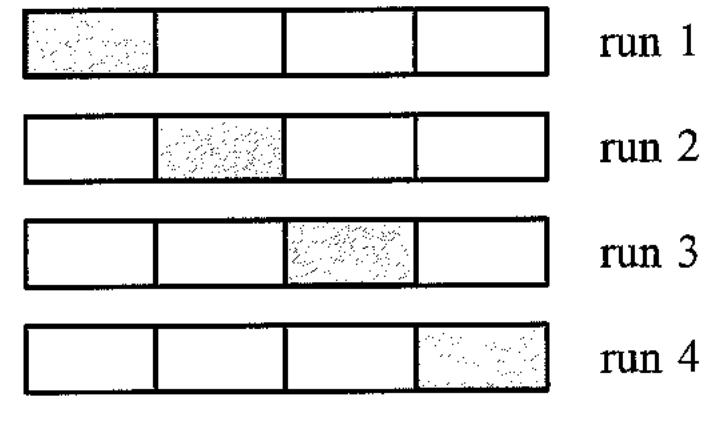
\includegraphics[width=0.55\textwidth]{ch01-fig1-12-cross-validation.png}
  \caption{$S$ 折交叉验证技术（这里以 $S=4$ 为例）的操作，首先将可用数据分成 $S$ 个等大小的子集。然后使用 $S-1$ 个子集来训练一组模型，并在剩余的子集上评估模型性能。接下来，将 $S$ 个子集中的每个子集作为保留集（图中红色块所示）重复上述过程，最后对 $S$ 次运行的性能评分取平均值}
  \label{figure:ch01-交叉验证}
\end{figure}

\begin{definition}[交叉验证]\label{definition:ch01-交叉验证}
设 $\mathcal{D}=\{(x_n,t_n)\}_{n=1}^{N}$ 为数据集，$S\in\mathbb{N}$ 且 $2\leqslant S\leqslant N$，$\{\mathcal{D}_{1},\cdots,\mathcal{D}_{S}\}$ 为 $\mathcal{D}$ 的一个划分，即 $\bigcup_{s=1}^{S}\mathcal{D}_{s}=\mathcal{D}$，且 $s\neq s'$ 时 $\mathcal{D}_{s}\cap\mathcal{D}_{s'}=\varnothing$，各折的样本数满足 $\bigl\lvert\,\lvert\mathcal{D}_{s}\rvert-\lvert\mathcal{D}_{s'}\rvert\,\bigr\rvert\leqslant1$。设 $\mathcal{A}$ 为学习算法，$\ell:\mathcal{Y}\times\mathcal{Y}\to[0,\infty)$ 为损失函数，并记
\begin{align*}
  \widehat{R}_{s}=\frac{1}{\lvert\mathcal{D}_{s}\rvert}\sum_{(x,t)\in\mathcal{D}_{s}}\ell\bigl(y(x;\mathcal{A}(\mathcal{D}\setminus\mathcal{D}_{s})),t\bigr),
  \qquad s=1,\cdots,S .
\end{align*}
若以平均值 $\frac{1}{S}\sum_{s=1}^{S}\widehat{R}_{s}$ 作为模型或超参数设置的评分，则这一过程称为\textbf{$S$ 折交叉验证}（$S$-fold cross-validation）；当 $S=N$ 时每一折恰含一个样本，该过程称为\textbf{留一法}（leave-one-out）。
\end{definition}

% SUPPLEMENT: parent=definition:ch01-交叉验证; kind=motivation; location=紧随其后的 remark
\begin{remark}
交叉验证解决的是“验证集太小则评估偏差大、验证集太大则训练数据不足”这对矛盾：每一折都让 $(S-1)/S$ 的数据参与训练，同时 $S$ 次评估覆盖了全部数据，因此既充分利用了数据，又给出了比单次划分更稳定的评分。
代价是训练次数增加为 $S$ 倍（\cref{figure:ch01-交叉验证}中的四次运行对应 $S=4$）。当 $S=N$ 时训练次数等于样本数，评估偏差最小但计算量最大；实际中常取 $S=5$ 或 $S=10$。此外，交叉验证假定各折数据可交换，若数据本身有分组或时间顺序，随机分折会破坏独立性，需要改用按组或按时间的划分。
\end{remark}

交叉验证的主要缺点在于所需的训练次数增加了 $S$ 倍，这对于训练过程本身计算成本较高的模型来说是一个大问题。交叉验证等使用独立数据评估性能的技术还存在另一个问题，即对于单个模型可能存在多个复杂度超参数（例如，可能有多个正则化超参数）。在最坏的情况下，探索这些超参数设置的最佳组合可能需要指数级数量的训练次数。现代机器学习的前沿领域需要非常大的模型和大规模训练数据集。因此，超参数设置的探索空间有限，很大程度上依赖于从小模型获得的经验和启发式方法。

这个将多项式模型拟合到基于正弦函数生成的合成数据集的简单示例，阐释了机器学习领域的一些核心概念，在后续章节我们将进一步用这个示例进行讨论。然而，现实中的机器学习应用往往要复杂得多：首先，用于模型训练的数据集规模可能会非常庞大，数据量通常会高出几个数量级；其次，模型的输入变量的数量通常也会显著增加，例如，在图像分析领域，输入变量的规模可达百万量级，并且还可能伴随着多个输出变量。在这些应用中，将输出映射到输入的可学习函数通常由一类被称为神经网络的模型来表征，这些模型往往具有海量的参数，其数量甚至可以达到千亿的规模。此时，误差函数将表现为这些模型参数的复杂非线性函数，无法再通过闭式解的方式进行最小化，而必须借助迭代优化的方法，利用误差函数关于模型参数的导数信息来逐步逼近最优解。这对计算机硬件提出了更高的要求，并且在实际应用中不可避免地会引入相当高的计算成本。

\end{document}
